\section{Alignment Learning Framework}
\begin{figure*}[!t]
    \centering
    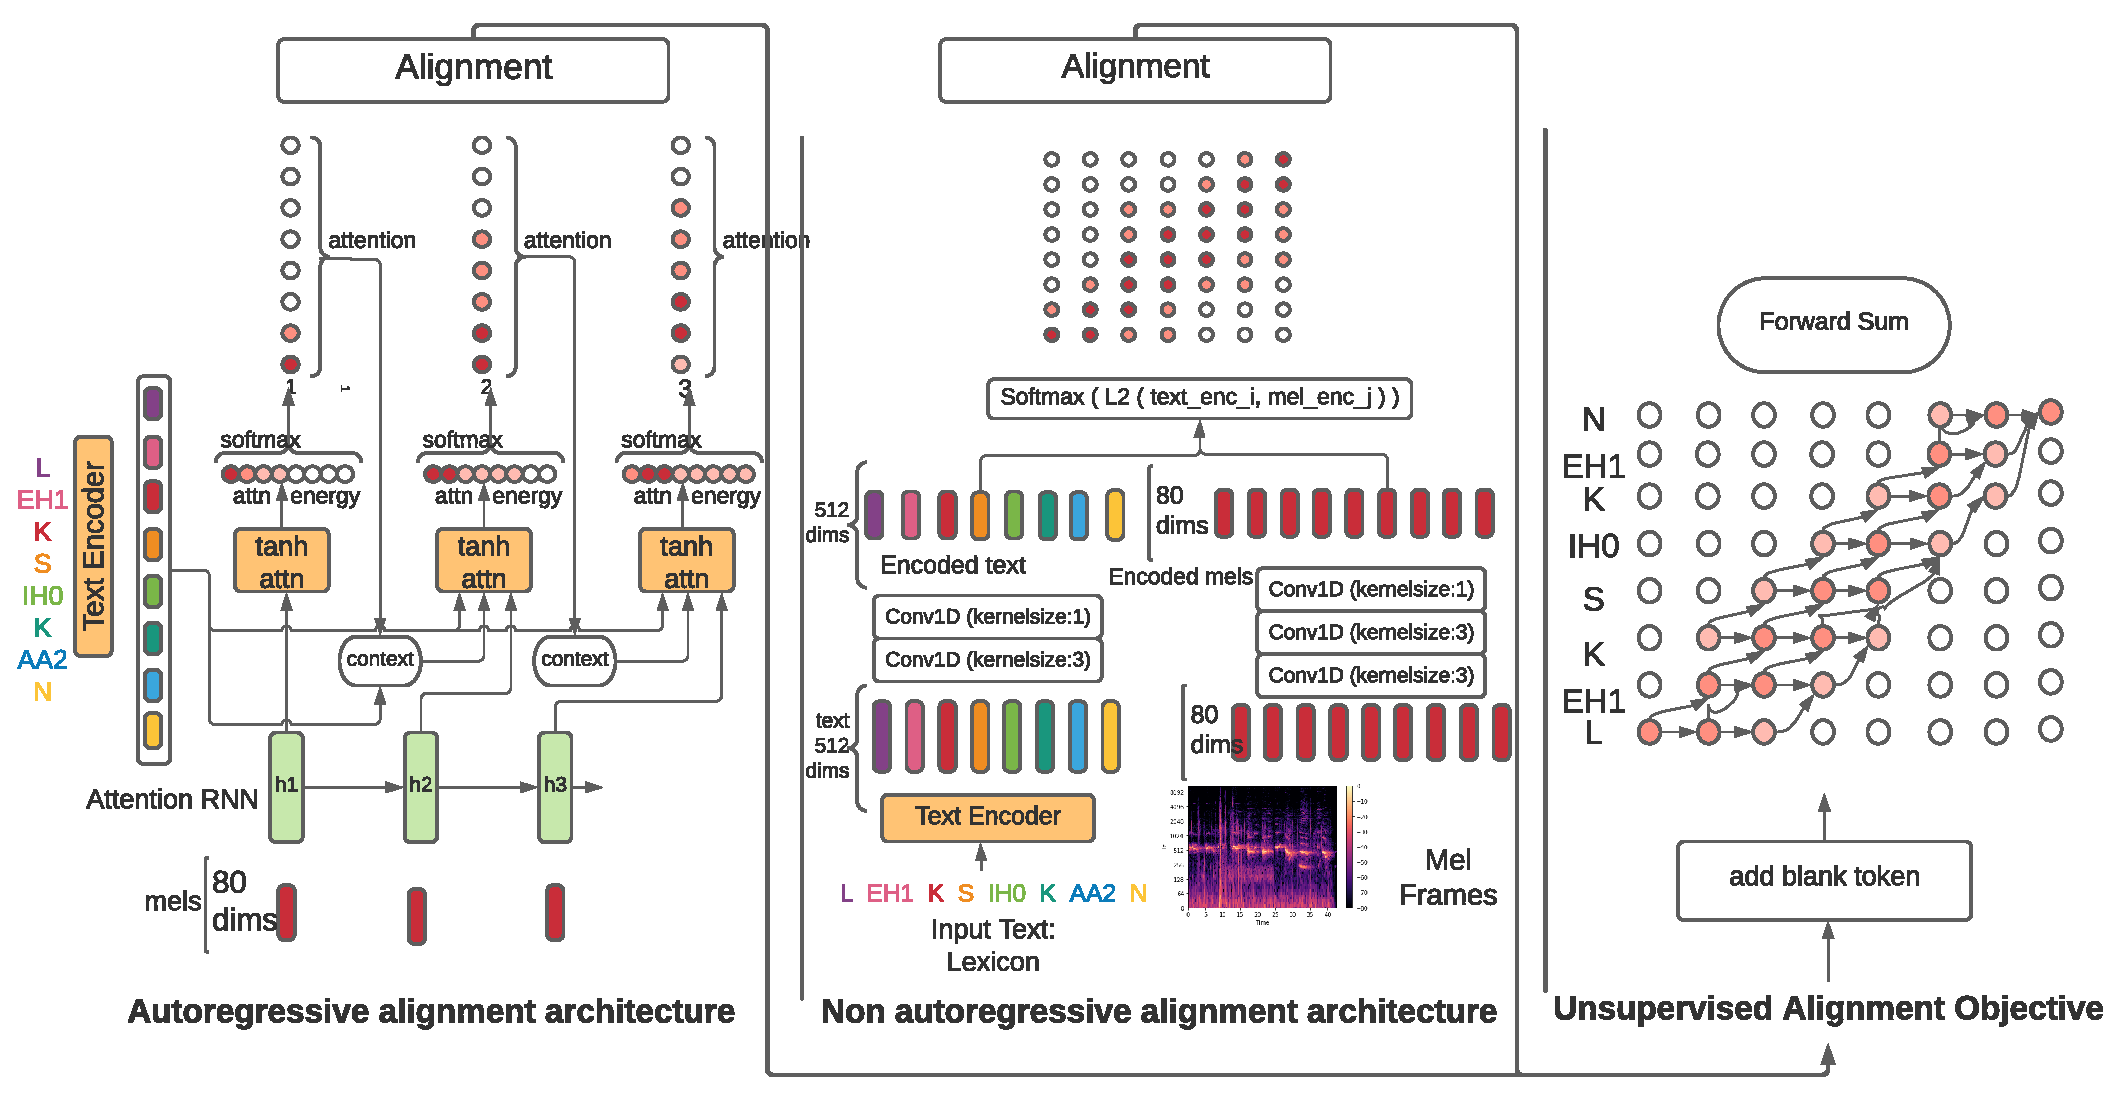
\includegraphics[width=0.9\linewidth]{images/OneTTSAlignmentToRuleThemAll.pdf}
    \vspace{-1em}
    \caption{Overview of our Alignment Learning Framework: autoregressive models use a sequential attention mechanism to generate alignments between text and mels. Non-autoregressive models encode text and mels using simple 1D convolutions and use pairwise $L_2$ distance to compute the alignments. The alignments represent the distribution $P(s_t | x_t)$ and the alignment objective (Equation \ref{eq:likelihood}).}
    \label{fig:alignment_arch}
    \vspace*{-0.5\baselineskip}
\end{figure*}

We extend the alignment learning approach proposed in RAD-TTS~\cite{rad_tts} to be more broadly applicable to various text to speech models especially autoregressive models. Our alignment framework is presented in Figure~\ref{fig:alignment_arch}. It takes the encoded text input $\Phi \in \mathbb{R}^{C_{\mathit{txt}} \times N}$ and aligns it to mel-spectrograms  $X \in \mathbb{R}^{C_{\mathit{mel}} \times T}$ where $T$ is number of mel frames and $N$ is the text length. In this section, we introduce the alignment learning objective and its application to autoregressive and parallel models.

\subsection{Unsupervised alignment learning objective}
\label{sec:ctc_objective}
To learn the alignment between mel-spectrograms $X$ and text $\Phi$, we use the alignment learning objective proposed in RAD-TTS~\cite{rad_tts}. This objective maximizes the likelihood of text given mel-spectrograms using the forward-sum algorithm used in Hidden Markov
Models (HMMs)~\cite{Rabiner89-ATO}. In our formulation, we constrain the alignment between text and speech to be monotonic, in order to avoid missing or repeating tokens. The following equation 
summarizes the likelihood of text given mels~\cite{rad_tts}:
%
% loss function  $\mathcal{L}_{\mathit{ForwardSum}}$ over model parameters $\theta$:
% \begin{align}\label{eq:likelihood}
%  \arg\min_\theta -P \left(S(\Phi) \mid X;\theta\right) = -\sum_{\mathbf{s} \in S(\Phi)} {\prod_{t=1}^{T}{P(s_t \mid x_t;\theta)} } ,
% \end{align}
%
\begin{align}\label{eq:likelihood}
 P \left(S(\Phi) \mid X;\theta\right) = \sum_{\mathbf{s} \in S(\Phi)} {\prod_{t=1}^{T}{P(s_t \mid x_t;\theta)} }
\end{align}
%
where $s$ is a specific alignment between mel-spectrograms and text (eg: $s1 = \phi_1, s2 = \phi_1, s3 = \phi_2, \ldots, sT = \phi_N$), $S(\Phi)$ is the set of all possible valid monotonic alignments, $ P(s_t | x_t)$ is the likelihood of a specific text token $s_t = \phi_i$ aligned for mel frame $x_t$ at timestep $t$. It is important to note that the above formulation of the alignment learning objective does not depend on how the likelihood  $P(s_t = \phi_i \mid x_t)$ is obtained. Hence, it can be applied to both autoregressive and parallel models. We define the forward sum objective that maximizes (\ref{eq:likelihood}) as $\mathcal{L}_{\mathit{ForwardSum}}$. 
Following RAD-TTS, we use an efficient, off-shelf CTC~\cite{ctc_icml2006} implementation to compute this objective (details in appendix of RAD-TTS~\cite{rad_tts}). 

\subsection{Autoregressive TTS Models}
\label{sec:autoregressive_alignment_framework}
Autoregressive TTS models typically use a sequential formulation of attention to learn online alignments. TTS models such as Tacotron~\cite{Tacotron} and Flowtron~\cite{Flowtron} use a content based attention mechanism that relies only on decoder inputs and the current attention hidden state to compute an attention map between encoder and decoder steps. Other autoregressive models use a location relative attention mechanism~\cite{locationattn} to promote forward movement of alignments~\cite{Tacotron2}. Although alignment learning in these autoregressive models is tightly coupled with the decoder and can be learned with the mel-spectrogram reconstruction objective, it has been observed that the likelihood of a misstep in the alignment increases with the length of the utterance. This results in catastrophic failure on long sequences and out-of-domain text~\cite{Battenberg}. The application of the unsupervised objective described in Sec \ref{sec:ctc_objective} improves both convergence speed during training and robustness during inference. 

Our autoregressive setup uses the standard stateful content based attention mechanism for Flowtron~\cite{Flowtron} and a hybrid attention mechanism that uses both content and location based features for Tacotron2~\cite{Tacotron2}. 
The location sensitive term (Eq. \ref{eq:location_term}) uses features computed from attention weights at previous decoder timesteps. 
We use a Tacotron2 encoder to obtain the sequence of encoded text representations $(\phi_i^{enc})_{i=1}^{N}$ and an attention RNN to produce a sequence of states $h_t$. A simple architecture is used to compute the alignment energies $e_{t, i}$ for text token $s_i$ at timestep $t$ for mel $x_t$ using the tanh attention~\cite{bahdanau2014neural}. The attention weights are computed with softmax over the text domain using the alignment energies. The following equations summarize the attention mechanism:
%
\begin{equation}
  \begin{aligned}
     (h_{{t}})_{t=1}^{T} = \text{RNN}(h_{t-1}, x_{t-1}, c_{t-1})
   \end{aligned}
\end{equation}
%
\begin{equation}
  \begin{aligned}
     c_{t} = \sum \alpha_{t, i}  \phi^{enc}_i 
   \end{aligned}
\end{equation}
%
\begin{equation}\label{eq:location_term}
  \begin{aligned}
     f_t = F (\alpha_{t-1})
   \end{aligned}
\end{equation}
%
\begin{equation}
  \begin{aligned}
     e_{t, i} = -v^{T} \tanh ( Wh_{t} + V\phi_i^{enc} + Uf_{t, i})
   \end{aligned}
\end{equation}
%
\begin{equation}
  \begin{aligned}
     P(s_t = \phi_i | x_t)= \alpha_{t, i} = Softmax(- e_t)_i,
   \end{aligned}
\end{equation}
%
where $f_t$ is the location relative term for location sensitive attention $F$ (cumulative attention from~\cite{Tacotron2} using a concatenation of the attention weights from the previous timestep and the cumulative attention weights). 
The attention weights model the distribution $P(s_t = \phi_i | x_t)$, which is exactly the right-most term in Equation (\ref{eq:likelihood}), and we incorporate it as the alignment loss:
\begin{equation}
  \begin{aligned}
     \mathcal{L}_{\mathit{align}} = \mathcal{L}_{\mathit{ForwardSum}}.
   \end{aligned}
\end{equation}

% We demonstrate in Section \ref{sec:experiments} that the addition of our proposed alignment objective makes the alignment module more robust, leading to better alignments and results in less pronunciation errors. 

\subsection{Parallel TTS Models}
\label{sec:non_autoregressive_alignment_framework}
As parallel TTS models have durations factored out from the decoder, the alignment learning module can be decoupled from the mel decoder as a standalone aligner. This provides a lot of flexibility in choosing the architecture to formulate the distribution $ P(s_t | x_t)$, where $s_t$ is a random variable for a text token aligned at timestep $t$ for mel frame $x_t$. Similar to GlowTTS~\cite{kim2020glowtts} and RAD-TTS~\cite{rad_tts}, we compute the soft alignment distribution based on the learned pairwise affinity between all text tokens and mel frames, which is normalized with softmax across the text domain

\begin{align}
    &D_{i,j} = dist_{L2}(\phi_i^{enc}, x_j^{enc}),\\
    &\attn{soft} = \texttt{softmax}(-D, \texttt{dim}=0).
\end{align}

We use two simple convolutional encoders from RAD-TTS~\cite{rad_tts} for encoding text $\Phi$ as $\Phi^{enc}$ and mel-spectograms $X$ as $X^{enc}$ with 2 and 3 1D convolution layers respectively. In Section \ref{sec:experiments}, we demonstrate that the same architecture works well with different parallel TTS models such as FastPitch and FastSpeech 2. Parallel models require alignments to be specified beforehand, typically in the form of the number of output samples for every input phoneme, equivalent to a binary alignment map. However, attention models produce soft alignment maps, constituting a train-test domain gap. Following~\cite{rad_tts,kim2020glowtts}, we use the Viterbi algorithm to find the most likely monotonic path through the soft alignment map in order to convert soft alignments ($\attn{soft}$) to hard alignments ($\attn{hard}$). We further close the gap between soft and hard alignments by forcing $\attn{soft}$ to match $\attn{hard}$ as much as possible by minimizing their KL-divergence. This is used in both Glow-TTS and RAD-TTS, formulated as ${L}_{bin}$:
\begin{equation}
    \mathcal{L}_{bin} = \attn{hard} \odot \log\attn{soft},
    %\vspace*{-\baselineskip}
\end{equation}
\begin{equation}
  \begin{aligned}
     \mathcal{L}_{\mathit{align}} = \mathcal{L}_{\mathit{ForwardSum}} + \mathcal{L}_{bin}.
   \end{aligned}
\end{equation}
where $\odot$ is Hadamard product, ${L}_{\mathit{align}}$ is final alignment loss.


% \subsection{Implementation of Forward Sum using CTC}
% \label{sec:ctc_implementation}
%  The CTC loss\cite{ctc_icml2006} has been widely used in speech recognition applications. In this section, we showcase how the CTC loss can be utilized to compute the forward sum objective $\mathcal{L}_{\mathit{ForwardSum}}$ that maximizes equation (\ref{eq:likelihood}). The CTC loss considers only monotonic transitions. 
 
\subsection{Alignment Acceleration}
\label{sec:accelerating_alignments}
Faster convergence of alignments means faster training for the full TTS model, as the decoder needs a stable alignment representation to build upon. During training, since the length of mel-spectrograms is known, we use a static 2D prior~\cite{rad_tts}, that is wider near the center and narrower near the corners to accelerate the alignment. This idea has been previously explored by Tachibana et al~\cite{guidedloss} where they introduce a new loss promoting near-diagonal alignments. Although our formulation with the 2D static prior is slightly different than Tachibana et al~\cite{guidedloss}, but we believe both should yield similar results. The 2D prior substantially accelerates the alignment learning by making far-off-diagonal elements less probable, although other priors can also be used for this goal. We apply this prior $f_{B}$ over the alignment $P(s \mid X \slimeq x_t)$ to obtain the following posterior:
 \begin{multline}
     f_{B}(k, \alpha, \beta) = {N \choose k} \frac{B(k + \alpha)B(N-k+\beta)}{B(\alpha, \beta)} 
 \end{multline}
 \begin{multline}
 P_{posterior}(\Phi \slimeq \phi_{k} \mid X\slimeq x_t)=\\
     P(\Phi \slimeq \phi_{k} \mid X\slimeq x_t) \odot f_{B}(k, \omega  t,  \omega  (T-t+1))
\end{multline}
 for $k=\{0,\ldots,N\}$, where $\alpha$, $\beta$ are hyperparameters of beta function $B(\cdot, \cdot)$, $N$ is number of tokens and $\omega$ is scaling factor controlling width of prior: lower the $\omega$, wider the width. 